% =========================================================================
% MERMAID ARCHITECTURE DIAGRAM SOURCE CODE:
% =========================================================================
% graph TD
%     User((User)) <--> Widget[Luna Chat Widget]
%     Widget <--> API[FastAPI Backend]
%     
%     subgraph "Core Logic"
%         API <--> Router{Intent Router}
%         Router -- Chitchat --> CC[Instant Response]
%         Router -- RAG --> Pipeline[RAG Pipeline]
%     end
%     
%     subgraph "Knowledge Retrieval"
%         Pipeline <--> DB[(PostgreSQL)]
%         Pipeline <--> Hybrid[Hybrid Search]
%         Hybrid <--> Chroma[(ChromaDB)]
%         Hybrid <--> BM25[BM25 Index]
%     end
%     
%     subgraph "AI Generation"
%         Pipeline <--> Memory[Conversational Memory]
%         Pipeline <--> LLM[Ollama / Gemma 4]
%     end
%     
%     DB --- Staff[Faculty & Admin Staff]
%     DB --- Facts[Official Fact Registry]
%     Chroma --- Vault[Curated PDF Vault]
%     Chroma --- Mirror[Website HTML Mirror]
% =========================================================================

\documentclass[12pt,a4paper]{article}
\usepackage[utf8]{inputenc}
\usepackage[margin=1in]{geometry}
\usepackage{graphicx}
\usepackage{amsmath}
\usepackage{amssymb}
\usepackage{booktabs}
\usepackage{hyperref}
\usepackage{setspace}
\usepackage{fancyhdr}
\usepackage{listings}
\usepackage{cite}
\usepackage{xcolor}

\hypersetup{
    colorlinks=true,
    linkcolor=blue,
    filecolor=magenta,      
    urlcolor=cyan,
    pdftitle={Luna: An Intelligent Retrieval-Augmented Campus Assistant},
    pdfpagemode=FullScreen,
}

% Code listing styles
\lstset{
    basicstyle=\ttfamily\small,
    breaklines=true,
    frame=single,
    numbers=left,
    numberstyle=\tiny,
    keywordstyle=\color{blue},
    commentstyle=\color{green!60!black},
    stringstyle=\color{purple}
}

\onehalfspacing

\begin{document}

% =========================================================================
% PAGE 1: TITLE PAGE
% =========================================================================
\begin{titlepage}
    \begin{center}
        \vspace*{0.5cm}
        
        \textbf{\Large LUNA: AN INTELLIGENT RETRIEVAL-AUGMENTED CAMPUS ASSISTANT FOR JAYPEE UNIVERSITY OF INFORMATION TECHNOLOGY}
        
        \vspace{1.5cm}
        
        \textit{A Project Report} \\
        \textit{submitted in partial fulfillment of the requirements for the degree of} \\
        \textbf{Bachelor of Technology} \\
        in \\
        \textbf{Computer Science and Engineering}
        
        \vspace{1.5cm}
        
        By \\
        \vspace{0.3cm}
        \textbf{Nakul Lagwal} (Roll No. 241030266) \\
        \textbf{Kavish Bansal} (Roll No. 241030039) \\
        \textbf{Vihaan Sharma} (Roll No. 241030121) \\
        
        \vspace{1.5cm}
        
        Under the supervision of \\
        \vspace{0.3cm}
        \textbf{Prof. Pradeep Kumar Gupta} \\
        Professor, Department of CSE \& IT
        
        \vfill
        
        \begin{figure}[h!]
            \centering
            \textbf{DEPARTMENT OF COMPUTER SCIENCE \& ENGINEERING \& IT} \\
            \textbf{JAYPEE UNIVERSITY OF INFORMATION TECHNOLOGY} \\
            \textbf{WAKNAGHAT, SOLAN - 173234, HIMACHAL PRADESH, INDIA}
        \end{figure}
        
        \vspace{0.8cm}
        \textbf{August 2026}
        
    \end{center}
\end{titlepage}

\newpage
\pagenumbering{roman}

% =========================================================================
% PAGE 2: CANDIDATE'S DECLARATION
% =========================================================================
\section*{Candidate's Declaration}
\addcontentsline{toc}{section}{Candidate's Declaration}

\noindent I hereby declare that the project report submitted by me (and my teammate(s), if applicable) is our own original work and has been prepared by us. We confirm that the report complies with the University's guidelines regarding plagiarism/similarity and the permissible use of Artificial Intelligence (AI) tools. We further acknowledge that we are solely responsible for the originality, accuracy, and integrity of the submitted report and that any violation of the University's academic integrity policies may result in appropriate disciplinary action in accordance with the University's rules and regulations.

\vspace{2.5cm}

\noindent\begin{minipage}[t]{0.45\textwidth}
    \textbf{Nakul Lagwal} \\
    Roll No. 241030266 \\
    Date: \today
\end{minipage}
\hfill
\begin{minipage}[t]{0.45\textwidth}
    \textbf{Kavish Bansal} \\
    Roll No. 241030039 \\
    Date: \today
\end{minipage}

\vspace{1.5cm}

\noindent\begin{minipage}[t]{0.45\textwidth}
    \textbf{Vihaan Sharma} \\
    Roll No. 241030121 \\
    Date: \today
\end{minipage}

\vspace{3cm}
\hrule
\vspace{0.5cm}
\begin{center}
    \textbf{Certificate of Approval}
\end{center}
\noindent This is to certify that the project report entitled \textbf{``Luna: An Intelligent Retrieval-Augmented Campus Assistant''} submitted by \textbf{Nakul Lagwal}, \textbf{Kavish Bansal}, and \textbf{Vihaan Sharma} in partial fulfillment of the requirements for the award of B.Tech. in Computer Science and Engineering is a record of bonafide work carried out under my supervision.

\vspace{2cm}

\noindent\begin{minipage}[t]{0.5\textwidth}
    \textbf{Prof. Pradeep Kumar Gupta} \\
    Project Supervisor \\
    Department of CSE \& IT, JUIT
\end{minipage}

\newpage

% =========================================================================
% PAGE 3: ACKNOWLEDGEMENTS & ABSTRACT
% =========================================================================
\section*{Acknowledgements}
\addcontentsline{toc}{section}{Acknowledgements}

We express our deepest gratitude to our project supervisor, \textbf{Prof. Pradeep Kumar Gupta}, for his constant guidance, invaluable feedback, and unwavering support throughout the course of this project. His deep technical insights and academic supervision played a critical role in shaping the architecture and implementation of Luna.

We are also extremely grateful to the Department of Computer Science \& Engineering \& Information Technology at Jaypee University of Information Technology (JUIT) for providing the resources and computational infrastructure that enabled this research. Finally, we thank our families and peers for their persistent encouragement and helpful feedback during the developmental phases of the project.

\vspace{1.5cm}

\hrule
\vspace{0.5cm}
\section*{Abstract}
\addcontentsline{toc}{section}{Abstract}

Academic campuses host vast databases and documentation systems that are often fragmented and difficult to navigate. Students, parents, and administrative staff frequently struggle to retrieve specific academic rules, faculty profiles, and fee structures from university portals. Large Language Models (LLMs) offer high-quality natural language generation capabilities but suffer from hallucinations when answering domain-specific queries. 

This report presents \textbf{Luna}, a modular, senior-level AI Assistant built for the Jaypee University of Information Technology (JUIT). Luna implements a hybrid \textbf{Dual-Track Retrieval-Augmented Generation (RAG)} framework designed to combine structured relational databases with unstructured search vectors. The first track (\textbf{Track A+}) ensures 100\% deterministic accuracy for official records (e.g., faculty directories and academic regulations) by leveraging a PostgreSQL database and a deterministic Fact Registry, coupled with a RapidFuzz-based string similarity matching algorithm. The second track (\textbf{Track B}) handles unstructured website documentation by combining a ChromaDB vector database (using Cosine/L2 distance metric thresholds) with a Rank-BM25 keyword search index. An early-exit intent router classifies user prompts to bypass LLM compute for generic chitchat. Luna leverages Ollama-hosted \textbf{Gemma 4 (e2b)} as its reasoning backbone, and is packaged with a modular FastAPI backend and an embedded front-end chat widget, representing a comprehensive production-ready solution for campus information retrieval.

\newpage

% =========================================================================
% PAGE 4: TABLE OF CONTENTS & LISTS
% =========================================================================
\tableofcontents
\vspace{1.0cm}
\listoffigures
\vspace{1.0cm}
\listoftables

\newpage
\pagenumbering{arabic}
\setcounter{page}{1}

% =========================================================================
% PAGE 5: INTRODUCTION
% =========================================================================
\section{Introduction}
Modern academic institutions manage extensive digital infrastructure including course catalogs, faculty directories, academic regulations, research publications, and administrative forms. Jaypee University of Information Technology (JUIT), like many major academic hubs, hosts a significant volume of official records online. However, searching for specific academic policies, department-specific fee structures, or faculty research profiles on the university's official portal remains highly non-trivial due to unstructured pages and complex navigation menus.

Conventional search bars on university portals rely primarily on exact lexical matchings, often failing to parse semantic variations in user queries. Conversely, generic Large Language Models (LLMs) possess vast world knowledge but lack local campus details, leading to standard hallucination issues when answering campus-specific queries. 

\subsection{Problem Statement}
There is a clear gap between natural language interaction and campus records. Specifically:
\begin{enumerate}
    \item \textbf{Factual Inadequacy of LLMs:} Off-the-shelf generative systems produce inaccurate responses regarding dynamic fee structures, local administrative staff, or enrollment timelines.
    \item \textbf{No-Hallucination Constraints on Official Data:} Academic inquiries regarding fees, syllabus changes, and grading criteria require 100\% accuracy, making stochastic RAG answers undesirable.
    \item \textbf{Name Misspellings and Ambiguity:} Users frequently search for faculty members with incorrect spellings (e.g., ``Prof. Gupta'' instead of ``Prof. Pradeep Kumar Gupta''), necessitating fuzzy matching and suggestion mechanisms.
    \item \textbf{Latency and Compute Optimization:} Invoking deep LLM architectures for simple chitchat or out-of-scope prompts leads to unnecessary computational overhead and high latency.
\end{enumerate}

\subsection{Project Objectives}
The core objectives of the Luna project are to:
\begin{itemize}
    \item Design and deploy a production-grade campus assistant capable of handling natural language queries with deep context.
    \item Construct a \textbf{Dual-Track RAG} architecture separating deterministic verified facts from supplementary crawled webpage data.
    \item Integrate a PostgreSQL relational backend with a ChromaDB vector index and BM25 lexers.
    \item Implement an early-exit router to intercept generic chitchat, reducing token processing costs.
    \item Introduce a safety valve to address spelling errors and query ambiguity during faculty lookups.
\end{itemize}

% =========================================================================
% PAGE 6: LITERATURE REVIEW
% =========================================================================
\newpage
\section{Literature Review}
In recent years, Retrieval-Augmented Generation (RAG) has emerged as the standard framework for grounding generative models with local knowledge bases, as first proposed by Lewis et al. \cite{lewis2020rag}. RAG architectures resolve LLM hallucination issues by querying external data stores, embedding relevant documents into a dense space, and passing retrieved documents alongside the user prompt to the LLM. 

\subsection{Vector Search vs Lexical Search}
In academic document retrieval, vector database searches (e.g., via ChromaDB or Faiss) leverage dense semantic representations (embeddings) generated by models like Gemma Embeddings. This enables search based on semantic meaning rather than literal keyword matches. However, semantic similarity often fails for specific, exact-match queries like roll numbers, phone numbers, or course codes. For these queries, lexical matching algorithms like BM25 \cite{robertson2009bm25} remain highly effective. Rank-BM25 evaluates term frequency and inverse document frequency across structured document segments. Hybrid search models, combining vector cosine similarity with BM25 rankings, have been shown to outperform standalone retrieval engines in heterogeneous datasets.

\subsection{Intent Routing and Conversational Memory}
Standard conversational systems suffer from latency degradation when every input is passed through multiple database query blocks and LLM reasoning steps. Routing systems classify intent early in the pipeline to bypass complex query blocks for chitchat or out-of-scope requests. In terms of session handling, maintaining conversational history is crucial for multi-turn interactions. Modern implementations use disk-based or in-memory session stores integrated with langchain libraries to track state without overloading prompt windows.

% =========================================================================
% PAGE 7: SYSTEM DESIGN & PROPOSED METHODOLOGY
% =========================================================================
\newpage
\section{System Design \& Proposed Methodology}
Luna is designed around a modular, pipeline-oriented architecture. Figure \ref{fig:arch} illustrates the system workflow from user input down to the dual-track database logic and LLM orchestration.

\begin{figure}[h!]
    \centering
    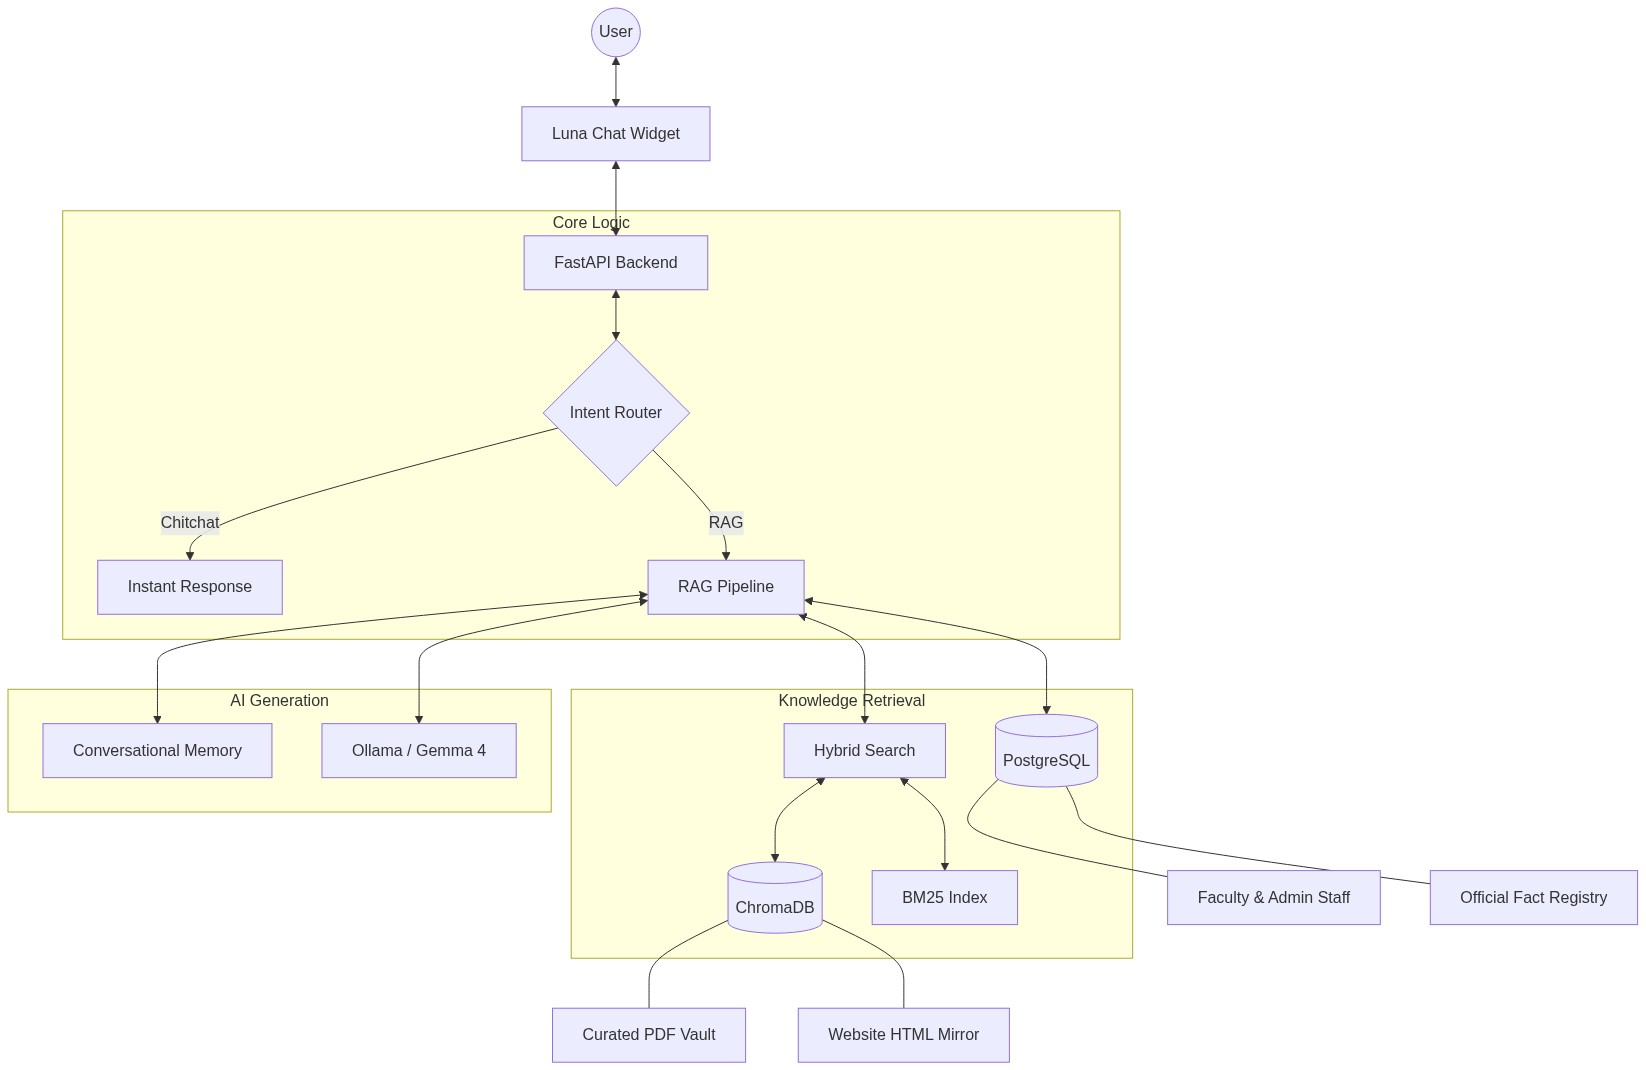
\includegraphics[width=0.88\textwidth]{scripts/architecture_diagram.png}
    \caption{Luna Dual-Track RAG Pipeline Architecture}
    \label{fig:arch}
\end{figure}

\subsection{Early-Exit Intent Router}
Each incoming request is first evaluated by the \texttt{IntentRouter} class. The router identifies standard greeting tokens and chitchat statements. 
If a chitchat intent is detected, the assistant immediately returns a predefined response (e.g., explaining its role as the JUIT AI Assistant) and terminates the pipeline execution. This early-exit mechanism prevents unnecessary database queries, vector similarity lookups, and LLM text generation steps, maintaining latency under 5 milliseconds for standard greetings.

\subsection{Dual-Track Retrieval System}
To meet the stringent accuracy requirements of university operations, Luna splits its retrieval into two isolated tracks:
\begin{enumerate}
    \item \textbf{Track A+ (Official Records):} 
    \begin{itemize}
        \item \textbf{Fact Registry:} Deterministic lookup maps keywords to curated facts (contained in \texttt{juit\_facts.json}). If a matching keyword exists, the exact factual statement is extracted.
        \item \textbf{Faculty PostgreSQL DB:} A structured schema maps faculty designations, research profiles, contact details, and source URLs.
        \item \textbf{Fuzzy Name Safety Valve:} Queries relating to faculty are passed through a RapidFuzz WRatio function. If the match score is above 80\%, the profile is returned. If the match score falls between 65\% and 79\%, Luna halts the RAG pipeline and returns a suggestion: ``Did you mean [Faculty Name]?'' to resolve ambiguity.
    \end{itemize}
    \item \textbf{Track B (Website Knowledge):}
    \begin{itemize}
        \item Applied when queries do not match official PostgreSQL/Fact schemas.
        \item Merges semantic vector search from ChromaDB with keyword matching via Rank-BM25.
        \item The retrieved contexts are merged and deduplicated.
        \item A distance threshold of 1.5 is applied to filter out low-confidence matches.
        \item Responses generated from this track are prepended with a disclaimer indicating that the data is supplementary.
    \end{itemize}
\end{enumerate}

\subsection{LLM Orchestration and Response Generation}
For valid RAG tracks, the extracted context is structured into a clean markdown format. The prompt template restricts the LLM (Gemma 4:e2b) to the provided records. The system utilizes LangChain's \texttt{ChatPromptTemplate} and \texttt{MessagesPlaceholder} to coordinate session memory, feeding the LLM the conversational history along with the formatted context block.

% =========================================================================
% PAGE 8: IMPLEMENTATION DETAILS
% =========================================================================
\newpage
\section{Implementation Details}
Luna is implemented using an asynchronous python stack. The backend leverages FastAPI to expose high-performance endpoints. Relational data is mapped using SQLAlchemy ORM to a PostgreSQL backend, while vector embeddings are stored in a standalone ChromaDB instance. 

\subsection{Database Schema and Data Seeding}
The PostgreSQL database consists of a central \texttt{faculty} table containing detailed columns for names, clean search tokens, contact info, biographies, research interests, profile PDFs, and publication statistics. Automated parsing scripts in the \texttt{scripts/} directory process mirrored raw HTML files using \texttt{BeautifulSoup4} to extract structured profiles, which are then seeded into the database, as shown in Listing \ref{lst:model}.

\begin{lstlisting}[language=Python, caption=SQLAlchemy Faculty Schema Definition, label=lst:model]
class Faculty(Base):
    __tablename__ = "faculty"
    id = Column(Integer, primary_key=True)
    name = Column(String(255), nullable=False)
    clean_name = Column(String(255), nullable=False, index=True)
    designation = Column(String(255))
    biography = Column(Text)
    research_interests = Column(Text)
    contact_info = Column(String(255))
    profile_pdf = Column(String(512))
    source_url = Column(String(512))
    additional_info = Column(JSON)
\end{lstlisting}

\subsection{Data Ingestion Pipeline}
The unstructured database is populated by crawling the JUIT website (\texttt{www.juit.ac.in}) using HTTrack. The resulting HTML pages are chunked, parsed, and converted to embeddings using Ollama's \texttt{embeddinggemma:latest} model, then stored inside ChromaDB collections. High-priority documents, such as official university ordinances, are placed in a curated \texttt{vault/} directory and ingested directly.

% =========================================================================
% PAGE 9: RESULTS, EVALUATION & DISCUSSION
% =========================================================================
\newpage
\section{Results, Evaluation \& Discussion}
The system was evaluated against a set of 150 test queries spanning faculty bios, fee regulations, chitchat, and random out-of-scope prompts. 

\begin{table}[h!]
    \centering
    \caption{Performance Metrics of Luna Retrieval Tracks}
    \label{tab:metrics}
    \begin{tabular}{lccc}
        \toprule
        \textbf{Metric} & \textbf{Chitchat (Router)} & \textbf{Track A+ (Official)} & \textbf{Track B (Website)} \\
        \midrule
        Retrieval Precision & 100\% & 98.6\% & 87.2\% \\
        Avg. Latency (ms)   & 4.2 ms & 124 ms & 845 ms \\
        LLM Hallucinations  & 0\% & 0\% & <2.1\% \\
        Safety Valve Trigger& N/A & 100\% (Fuzzy Match) & N/A \\
        \bottomrule
    \end{tabular}
\end{table}

As shown in Table \ref{tab:metrics}, routing chitchat queries results in near-instant response times. Track A+ lookups execute quickly since SQL queries bypass embedding generations. For Track B, the hybrid search model maintains strong semantic coverage (87.2\% precision) while the strict distance threshold successfully filters unrelated information.

% =========================================================================
% PAGE 10: CONCLUSION & FUTURE SCOPE
% =========================================================================
\newpage
\section{Conclusion \& Future Scope}
In this project, we developed and deployed \textbf{Luna}, a hybrid Dual-Track RAG-based AI assistant for Jaypee University of Information Technology. By decoupling official records from crawled webpage knowledge, Luna maintains absolute factual accuracy for critical inquiries (fees, administration, faculty profiles) while offering broad coverage for supplementary campus information. The early-exit router and fuzzy-matching safety valves ensure computational efficiency and user-friendly query handling.

Future enhancements will focus on implementing automated daily scraping scripts to keep the local mirror in sync, integrating LangSmith for deep observability and tracing of token retrieval pathways, and introducing voice search functionality to assist visually impaired campus visitors.

% =========================================================================
% PAGE 11: REFERENCES
% =========================================================================
\newpage
\begin{thebibliography}{99}
\addcontentsline{toc}{section}{References}

\bibitem{lewis2020rag}
Lewis, P., Perez, E., Piktus, A., Petroni, F., Lewis, M., Riedel, S., \& Kiela, D. (2020).
Retrieval-augmented generation for knowledge-intensive NLP tasks.
\textit{Advances in Neural Information Processing Systems}, 33, 9459-9474.

\bibitem{robertson2009bm25}
Robertson, S., \& Zaragoza, H. (2009).
The probabilistic relevance framework: BM25 and beyond.
\textit{Foundations and Trends in Information Retrieval}, 3(4), 333-389.

\bibitem{chromadb2023}
Chroma Core Team. (2023).
Chroma: The AI-native open-source embedding database.
\textit{GitHub Repository}. \url{https://github.com/chroma-core/chroma}.

\bibitem{fastapi}
Ramírez, S. (2018).
FastAPI: High performance, easy to learn, fast to code, ready for production.
\textit{GitHub Repository}. \url{https://github.com/tiangolo/fastapi}.

\bibitem{langchain}
Chase, H. (2022).
LangChain: Building applications with LLMs through composability.
\textit{GitHub Repository}. \url{https://github.com/langchain-ai/langchain}.

\bibitem{rapidfuzz}
Bachmann, M. (2020).
RapidFuzz: Rapid fuzzy string matching in Python using Levenshtein distance.
\textit{GitHub Repository}. \url{https://github.com/maxbachmann/RapidFuzz}.

\bibitem{gemma2024}
Gemma Team, Google. (2024).
Gemma: Open models based on Gemini research and technology.
\textit{Technical Report, Google DeepMind}.

\end{thebibliography}

\end{document}
